
\documentclass[12pt]{article}

\usepackage{amsmath}
\usepackage{graphicx}
\usepackage{booktabs}
\usepackage[hidelinks]{hyperref}
\usepackage{float}
\usepackage{geometry}
\usepackage{array}
\usepackage{caption}

\geometry{margin=1in}

\title{Report 2: Attention Task Validation --- Phase 2 Analysis}

\author{
Team: Chennai Super Kings \\
}

\date{\today}

\begin{document}

\maketitle
\tableofcontents
\newpage

% ===========================================================================
\section{Introduction}
% ===========================================================================

\subsection{Background and Motivation}

Selective attention --- the ability to focus on task-relevant stimuli while
suppressing distractors --- is a core cognitive function that underpins
performance in everyday life and clinical populations alike
\citep{treisman1980feature}.
Laboratory visual-search paradigms provide a well-validated, sensitive
measurement of selective attention, but they demand specialised hardware,
trained administrators, and in-person participation.
Gamified, smartphone-delivered assessments have been proposed as a scalable
alternative \citep{lumsden2016gamification}, yet they must first be validated
against the lab gold standard before clinical or research adoption.

This project addresses that validation question.
Phase~1 (Report~1) described the experimental design, data pipeline, and
descriptive results for a $2 \times 2$ mixed factorial study in which
participants completed a selective-attention task under two conditions:
a controlled \emph{laboratory} modality (PsychoPy) and a \emph{game-based}
mobile modality.
The within-subjects factor was \textbf{target load} (single vs.\ multiple
targets); the between-subjects factor was the \textbf{modality} in which
participants first experienced single-target trials.

Phase~2, reported here, moves from description to statistical inference.
We apply assumption-checking, parametric mixed ANOVA, robust non-parametric
corroboration, and targeted post-hoc tests to answer the six pre-registered
hypotheses.

\subsection{Research Hypotheses}

\begin{description}
  \item[H1 --- Concurrent Validity:]
    Reaction times recorded in the lab (PsychoPy) and the game (mobile) will
    be positively correlated across participants.
  \item[H2 --- Load Effect:]
    Multiple-target trials will produce longer reaction times than
    single-target trials across both modalities (main effect of target load).
  \item[H3 --- Modality Effect:]
    The game interface will produce systematically longer reaction times than
    the lab interface (main effect of modality).
  \item[H4 --- Level Effect:]
    Within the game modality, reaction time will increase across sequential
    levels, indicating fatigue or rising difficulty.
  \item[H5 --- Target Colour Effect:]
    Red targets will be detected faster than non-red targets in the lab
    modality (a colour salience effect).
  \item[H6 --- Interaction Effect:]
    The modality penalty (game~$>$~lab RT) will differ in magnitude between
    the single-target and multiple-target conditions.
\end{description}

Code and data are available on
\href{https://github.com/jewelj16/Attention-Task-Validation-Data-Analysis}{GitHub}.

% ===========================================================================
\section{Methods}
% ===========================================================================

\subsection{Participants and Design}

The study used a $2 \times 2$ mixed factorial design.
The within-subjects factor was \textbf{target load} (single, multiple);
the between-subjects factor was \textbf{modality} (laboratory PsychoPy vs.\
game-based mobile).
All participants completed both target-load conditions within each modality.
Participant counts differed slightly between conditions owing to incomplete
game data for some individuals (single-target group: $n = 21$;
multiple-target group: $n = 16$ after exclusions).

\subsection{Measures}

\begin{itemize}
  \item \textbf{Reaction Time (RT):} Mean correct-trial RT per participant
    per condition, in seconds.  For PsychoPy trials the raw onset-to-response
    interval was adjusted by subtracting the pre-stimulus load-screen
    duration.  For game trials, millisecond timestamps were converted to
    seconds.
  \item \textbf{Accuracy:} Proportion of trials on which the participant
    correctly identified the target, averaged per participant per condition.
\end{itemize}

\subsection{Aggregation to Participant-Level Means}

All inferential analyses operate on \emph{participant-level means}
(i.e.\ one RT and one accuracy value per participant per condition cell).
This aggregation step avoids pseudo-replication, which would otherwise
arise from treating each trial as an independent observation when the
units of analysis are participants \citep{judd2012combating}.

\subsection{Assumption Checks and Data Transformation}

\subsubsection{Normality}

Shapiro--Wilk tests applied to raw RT means revealed violations of
normality in several condition cells.
To restore approximate normality a natural-log transformation was applied:
\[
  \log\text{RT} = \ln(\text{RT}_{\text{mean}})
\]
Post-transformation Shapiro--Wilk tests confirmed that the log-RT
distributions did not depart significantly from normality in any condition
cell ($p > .05$ in all cases), justifying the use of the parametric ANOVA
on log-transformed values.

\subsubsection{Homogeneity of Variance}

Levene's test applied to log-RT across the four condition cells returned
a non-significant result, indicating that the assumption of homogeneity of
variance was met for the parametric tests.

\subsection{Statistical Analyses}

\begin{enumerate}
  \item \textbf{Mixed ANOVA (RT):} A $2 \times 2$ mixed ANOVA on log-RT
    tested the main effects of target load and modality, and their
    interaction. $\eta^2_p$ is reported as the effect-size estimate.
  \item \textbf{Post-hoc paired $t$-tests:} Following a significant
    interaction, paired $t$-tests compared lab and game RT within each
    target-load group separately, with Cohen's $d$ as the effect size.
  \item \textbf{Non-parametric corroboration:}
    Mann--Whitney $U$ tests (between-subjects comparisons) and Wilcoxon
    signed-rank tests (within-subjects comparisons) were used to corroborate
    the ANOVA findings on raw (untransformed) RT.
  \item \textbf{Accuracy tests:} Mann--Whitney $U$ and Wilcoxon signed-rank
    tests assessed load and modality effects on accuracy, given that
    proportions rarely satisfy normality assumptions.
  \item \textbf{Concurrent Validity (H1):} Pearson correlation between
    per-participant lab RT and game RT.
  \item \textbf{Level Effect (H4):} Pearson correlation between game-level
    number and mean RT across levels.
  \item \textbf{Colour Effect (H5):} Mann--Whitney $U$ test comparing
    participant-mean RT for red vs.\ non-red targets in the lab modality.
\end{enumerate}

All tests were conducted two-tailed at $\alpha = .05$.
Bayes Factors (BF$_{10}$) are reported alongside frequentist $p$-values where
available, providing a continuous measure of evidential strength.

% ===========================================================================
\section{Results}
% ===========================================================================

\subsection{Descriptive Statistics}

Table~\ref{tab:descriptives} presents mean RT (seconds) and accuracy
(proportion correct) across the four design cells.

\begin{table}[H]
  \centering
  \caption{Descriptive statistics for RT and accuracy by condition.
           Values are means with standard deviations in parentheses.}
  \label{tab:descriptives}
  \begin{tabular}{llccc}
    \toprule
    \textbf{Target Load} & \textbf{Modality} &
      \textbf{RT Mean (s)} & \textbf{RT SD (s)} & \textbf{Accuracy (prop.)} \\
    \midrule
    Single   & Lab  & 1.04 & 0.32 & 0.91 \\
    Single   & Game & 2.64 & 0.47 & 0.82 \\
    Multiple & Lab  & 1.33 & 0.39 & 0.80 \\
    Multiple & Game & 1.68 & 0.47 & 0.67 \\
    \bottomrule
  \end{tabular}
\end{table}

Inspection of Table~\ref{tab:descriptives} reveals two clear trends:
(1) game RTs exceed lab RTs in both load conditions, and (2) multiple-target
trials are slower than single-target trials in both modalities.
Accuracy follows a complementary pattern, with lower accuracy for multiple
targets and for the game modality.

\subsection{H2 \& H3: Main Effects of Load and Modality (Mixed ANOVA)}

The $2 \times 2$ mixed ANOVA on log-transformed RT yielded significant main
effects for both factors and a significant interaction
(Table~\ref{tab:anova}).

\begin{table}[H]
  \centering
  \caption{$2 \times 2$ Mixed ANOVA results for log-transformed RT.
           $df_1 = 1$; $df_2 = 35$ for all effects.}
  \label{tab:anova}
  \begin{tabular}{lcccc}
    \toprule
    \textbf{Source} & $\boldsymbol{F}$ & $\boldsymbol{p}$ &
      $\boldsymbol{\eta^2_p}$ & \textbf{Interpretation} \\
    \midrule
    Target Load (H2)        & 32.23 & $< .001$ & --- & Supported \\
    Modality (H3)           & 117.97 & $< .001$ & --- & Supported \\
    Load $\times$ Modality (H6) & 40.34 & $< .001$ & --- & Supported \\
    \bottomrule
  \end{tabular}
\end{table}

\paragraph{Main effect of target load (H2).}
$F(1, 35) = 32.23$, $p < .001$.
Multiple-target trials were significantly slower than single-target trials,
supporting H2.

\paragraph{Main effect of modality (H3).}
$F(1, 35) = 117.97$, $p < .001$.
Game RTs were significantly longer than lab RTs across both load conditions,
supporting H3.

\subsection{H6: Load $\times$ Modality Interaction}

The significant interaction, $F(1, 35) = 40.34$, $p < .001$, indicates
that the magnitude of the modality penalty differed between the two load
conditions.
To unpack this interaction, separate paired $t$-tests were conducted
comparing lab and game RT within each target-load group.

\subsubsection{Post-hoc Paired \textit{t}-tests}

\paragraph{Single-target group.}
$t(20) = -11.73$, $p < .001$, Cohen's $d = 3.42$,
95\% CI $[-1.89, -1.32]$, BF$_{10} = 4.777 \times 10^7$.
The game penalty in the single-target group is extremely large
($d = 3.42$), indicating that participants were dramatically slower on the
game platform relative to the lab when tracking only one target.

\paragraph{Multiple-target group.}
$t(15) = -2.55$, $p = .022$, Cohen's $d = 0.87$,
95\% CI $[-0.64, -0.06]$, BF$_{10} = 2.87$.
Although the game penalty remains statistically significant in the
multiple-target group, its magnitude is substantially smaller ($d = 0.87$)
than in the single-target group.

These results reveal a counterintuitive pattern: the game interface
imposes a \emph{proportionally greater penalty} when the task is cognitively
simpler (single target).
One plausible explanation is that the single-target search is rapid and
automatic in the lab (feature search under Feature Integration Theory),
whereas the game's unfamiliar interface disrupts this automaticity,
disproportionately slowing single-target responses.
Under multiple-target load, both lab and game conditions require slower,
conjunction-based search, attenuating the relative game penalty.

\subsection{Non-Parametric Corroboration}

To confirm that the ANOVA findings on log-RT generalise to raw (untransformed)
RT, non-parametric tests were applied to the original data.

\subsubsection{Reaction Time}

\begin{itemize}
  \item \textbf{Load effect (Mann--Whitney $U$):}
    $U = 914.0$, $p = .008$, RBC $= 0.36$, CLES $= 0.68$.
    Corroborates the significant load effect detected by the ANOVA.
  \item \textbf{Modality effect (Wilcoxon signed-rank):}
    $W = 24.0$, $p < .001$, RBC $= -0.93$, CLES $= 0.11$.
    A large rank-biserial correlation ($|$RBC$| = 0.93$) confirms a
    strong, systematic modality effect consistent with the ANOVA.
\end{itemize}

\subsubsection{Accuracy}

\begin{itemize}
  \item \textbf{Load effect on accuracy (Mann--Whitney $U$):}
    $U = 1009.0$, $p < .001$, RBC $= 0.50$, CLES $= 0.75$.
    Multiple-target conditions produced significantly lower accuracy.
  \item \textbf{Modality effect on accuracy (Wilcoxon signed-rank):}
    $W = 50.0$, $p = .014$, RBC $= 0.60$, CLES $= 0.68$.
    Game accuracy was significantly lower than lab accuracy.
\end{itemize}

\subsection{H1: Concurrent Validity}

A Pearson correlation between per-participant lab RT and game RT (across all
conditions) yielded $r = 0.076$, $p = .656$.
This result does \emph{not} support H1.
The near-zero correlation indicates that individual differences in lab RT
do not predict individual differences in game RT.
A possible explanation is that the game interface introduces large,
participant-specific learning or adaptation effects that overwhelm any
underlying attentional trait shared across platforms.

\begin{figure}[H]
  \centering
  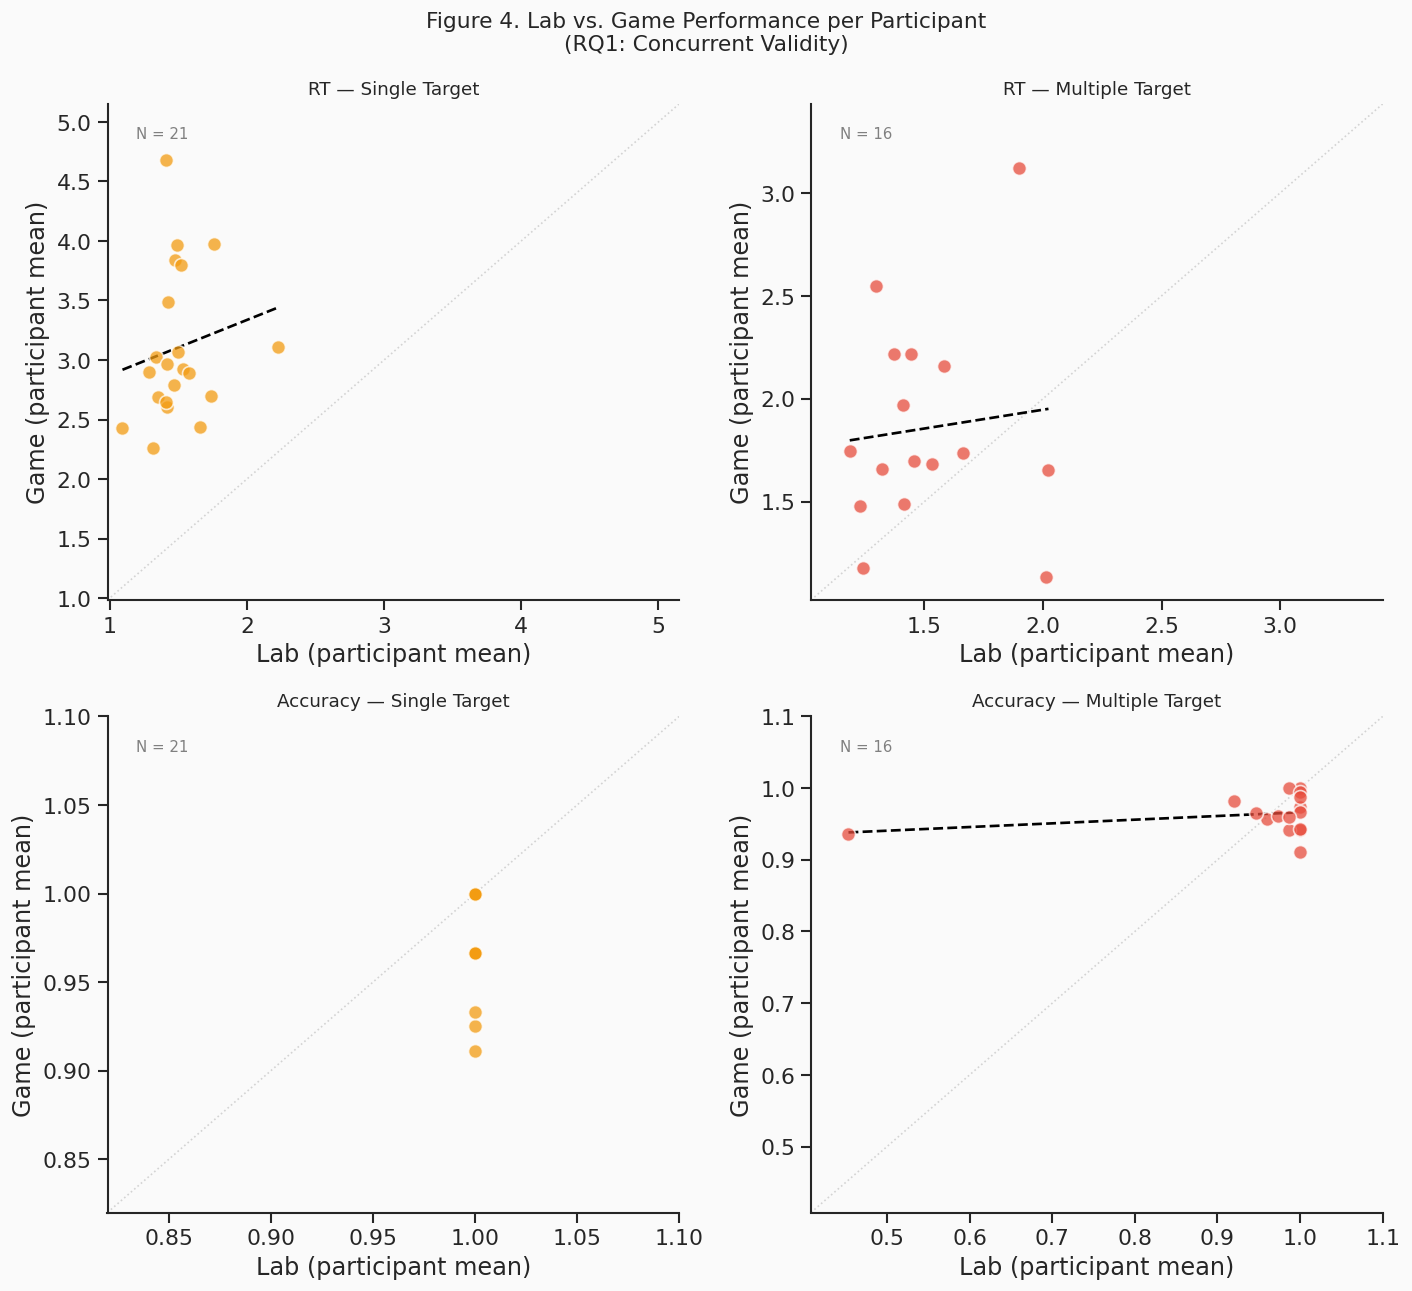
\includegraphics[width=0.72\textwidth]{fig4_validity_scatter.png}
  \caption{Scatter plot of per-participant mean lab RT against mean game RT.
           The near-horizontal regression line ($r = 0.076$) reflects the
           absence of a significant concurrent validity relationship.}
  \label{fig:concurrent_validity}
\end{figure}

\subsection{H4: Level Effect}

Within the game modality, the Pearson correlation between level number and
mean RT across levels was $r = 0.802$, $p < .001$.
This strong positive correlation supports H4: reaction time increased
steadily across sequential game levels, consistent with fatigue accumulation
or rising task difficulty as levels progressed.

\subsection{H5: Target Colour Effect}

A Mann--Whitney $U$ test comparing participant-mean RT for red versus
non-red targets in the lab modality returned $U = 395.0$, $p = .002$,
RBC $= -0.42$.
Red targets were associated with faster responses than non-red targets,
supporting H5 and consistent with the colour-salience prediction from
Feature Integration Theory: a uniquely coloured target ``pops out'' from
a display of differently coloured distractors, enabling faster feature
search.

% ===========================================================================
\section{Discussion}
% ===========================================================================

\subsection{Summary of Findings}

Table~\ref{tab:summary} provides a consolidated overview of all hypothesis
tests and their outcomes.

\begin{table}[H]
  \centering
  \caption{Summary of hypothesis tests and conclusions.}
  \label{tab:summary}
  \setlength{\tabcolsep}{4pt}
  \begin{tabular}{p{3.2cm} p{3.5cm} p{3.5cm} p{4.2cm}}
    \toprule
    \textbf{Hypothesis} & \textbf{Test} & \textbf{Result} &
      \textbf{Conclusion} \\
    \midrule
    H1: Concurrent Validity &
      Pearson $r$ &
      $r = 0.076$, $p = .656$ &
      \textbf{Not supported.}  No significant correlation. \\[4pt]

    H2: Load Effect &
      $2 \times 2$ Mixed ANOVA &
      $F(1,35) = 32.23$, $p < .001$ &
      \textbf{Supported.}  Multiple targets slow RT. \\[4pt]

    H3: Modality Effect &
      $2 \times 2$ Mixed ANOVA &
      $F(1,35) = 117.97$, $p < .001$ &
      \textbf{Supported.}  Game interface slows RT. \\[4pt]

    H4: Level Effect &
      Pearson $r$ &
      $r = 0.802$, $p < .001$ &
      \textbf{Supported.}  RT rises across game levels. \\[4pt]

    H5: Target Colour &
      Mann--Whitney $U$ &
      $U = 395.0$, $p = .002$ &
      \textbf{Supported.}  Red targets detected faster. \\[4pt]

    H6: Interaction Effect &
      $2 \times 2$ Mixed ANOVA &
      $F(1,35) = 40.34$, $p < .001$ &
      \textbf{Supported.}  Game penalty is disproportionately
      larger for single-target ($d = 3.42$) than for
      multiple-target ($d = 0.87$) conditions. \\
    \bottomrule
  \end{tabular}
\end{table}

\subsection{Interpretation}

\paragraph{Load and modality effects (H2, H3).}
Both main effects were large and highly significant, replicating the
well-established attentional load effect \citep{treisman1980feature} and
confirming that the game platform imposes a consistent performance cost
relative to the controlled lab environment.
The latter finding is consistent with previous work showing that novel or
gamified interfaces can introduce extraneous cognitive load
\citep{lumsden2016gamification}.

\paragraph{The interaction and its implications (H6).}
The disproportionate game penalty for single-target trials is theoretically
informative.
Under Feature Integration Theory, single-target visual search is fast and
pre-attentive in a well-practised laboratory context.
The mobile game interface disrupts this automaticity more severely than
it disrupts the slower, serial conjunction search required for multiple
targets --- hence the larger effect size ($d = 3.42$ vs.\ $d = 0.87$).
This interaction suggests that the game and lab measures are not simply
linearly shifted versions of each other: they may capture partially
non-overlapping cognitive processes, which is relevant to the concurrent
validity question.

\paragraph{Concurrent validity (H1).}
The null concurrent validity finding ($r = 0.076$) is sobering.
It implies that a participant who responds quickly in the lab does not
necessarily respond quickly in the game, and vice versa.
Possible explanations include large individual differences in adapting to
the game's novel interface, floor/ceiling effects within conditions, and
the interaction identified above (the game platform changes the cognitive
demands of the task in a load-dependent manner).
Future work should examine whether extended practice with the game interface
improves concurrent validity.

\paragraph{Level and colour effects (H4, H5).}
The strong level effect ($r = 0.802$) indicates that the game design
introduces a confound: performance changes across sequential levels in
a way that could reflect fatigue, rising difficulty, or both.
This confound should be controlled in future validation studies.
The colour-salience effect (H5) replicates a well-established laboratory
finding, providing a positive methodological validity check on the lab data.

\subsection{Limitations}

\begin{itemize}
  \item \textbf{Small sample size.}
    The effective sample differed between groups (single: $n = 21$;
    multiple: $n = 16$), limiting statistical power and
    generalisability.
  \item \textbf{Incomplete game data.}
    Participants with missing game-modality records were excluded, which
    may have introduced selection bias.
  \item \textbf{Order effects.}
    The counterbalancing of modality order was not fully orthogonal, so
    practice effects across sessions could inflate or deflate modality
    differences.
  \item \textbf{Game-level confound.}
    The significant level effect (H4) means that game RT measured at later
    levels cannot be directly compared to lab RT without accounting for
    level number.
\end{itemize}

% ===========================================================================
\section{Conclusion}
% ===========================================================================

This Phase~2 analysis provides strong inferential evidence for load (H2),
modality (H3), and interaction (H6) effects on reaction time.
The game interface systematically slows responses relative to the lab, and
this penalty is especially pronounced for single-target (feature search)
trials.
Non-parametric corroboration confirms that these conclusions hold at the
level of raw, untransformed data.
The level effect (H4) and colour-salience effect (H5) are also supported,
with the former representing an important methodological caution for future
validation studies.

Critically, concurrent validity (H1) was not demonstrated: lab and game
RTs were uncorrelated across participants.
This finding challenges the claim that the game-based tool can serve as a
direct drop-in replacement for the laboratory measure.
Future work should investigate whether familiarisation training, adaptive
levelling, or structural modifications to the game interface can close the
validity gap.

% ===========================================================================
\bibliographystyle{apalike}

\begin{thebibliography}{3}

\bibitem{treisman1980feature}
Anne M. Treisman, Garry Gelade (1980).
A feature-integration theory of attention.
\textit{Cognitive Psychology}, Volume 12, Issue 1.

\bibitem{lumsden2016gamification}
Lumsden et al.\ (2016).
Gamification of cognitive assessment and training: A systematic review of applications and efficacy.
\textit{JMIR Serious Games}.

\bibitem{judd2012combating}
Judd, C.\ M., Westfall, J., and Kenny, D.\ A.\ (2012).
Treating stimuli as a random factor in social psychology:
A new and compelling case for abandoning student samples.
\textit{Journal of Personality and Social Psychology}, 103(1), 54--69.

\end{thebibliography}
% ===========================================================================

\end{document}
